\section{Sequence diagrams}

\subsection{Introduction}

\begin{flushleft}
Les sequences diagrams nous permettent de détailler le chemin effectué lorsqu'un utilisateur souhaite intéragir avec l'application.
\end{flushleft}

\begin{flushleft}
Dans le but de permettre une meilleure compréhension de ces diagrammes, nous les avons séparés en trois parties.
\begin{enumerate}
\item Common
\item Client
\item Provider
\end{enumerate}
\end{flushleft}

\begin{flushleft}
Afin de les réaliser convenablement, nous sommes repartis de notre class diagram et nos Use cases diagrams et avons représenté l'interaction des méthodes avec l'API et la base de données.
\end{flushleft}

\begin{flushleft}
Avant de commencer, il est important de signaler dans le but d'éviter toute répétition, que la vérification du token s'effectuera pour chaque action lorsqu'un utilisateur est connecté.
\end{flushleft}

\begin{flushleft}
Si le token est bon, on continue le programme, sinon, on envoie un message d'erreur à l'aide de la méthode "sendMessageError".
\end{flushleft}

\newpage
\subsection{Common}

\newpage
\subsection{Client}

\begin{flushleft}
Commençons par le Use Case \textbf{"Voir les contrats"}, nous appelons la méthode "getAllContract" de clientApi et ensuite, la méthode du même nom de ClientDB.
\end{flushleft}

\begin{flushleft}
Le but étant d'obtenir une ArrayList de "contractBasic", nous devons effecter une boucle afin de récupérer tous les "contractBasic".
\end{flushleft}

\begin{flushleft}
Une fois effectuée, nous renvoyons cette liste.
\end{flushleft}

\begin{figure}[h]
\centering
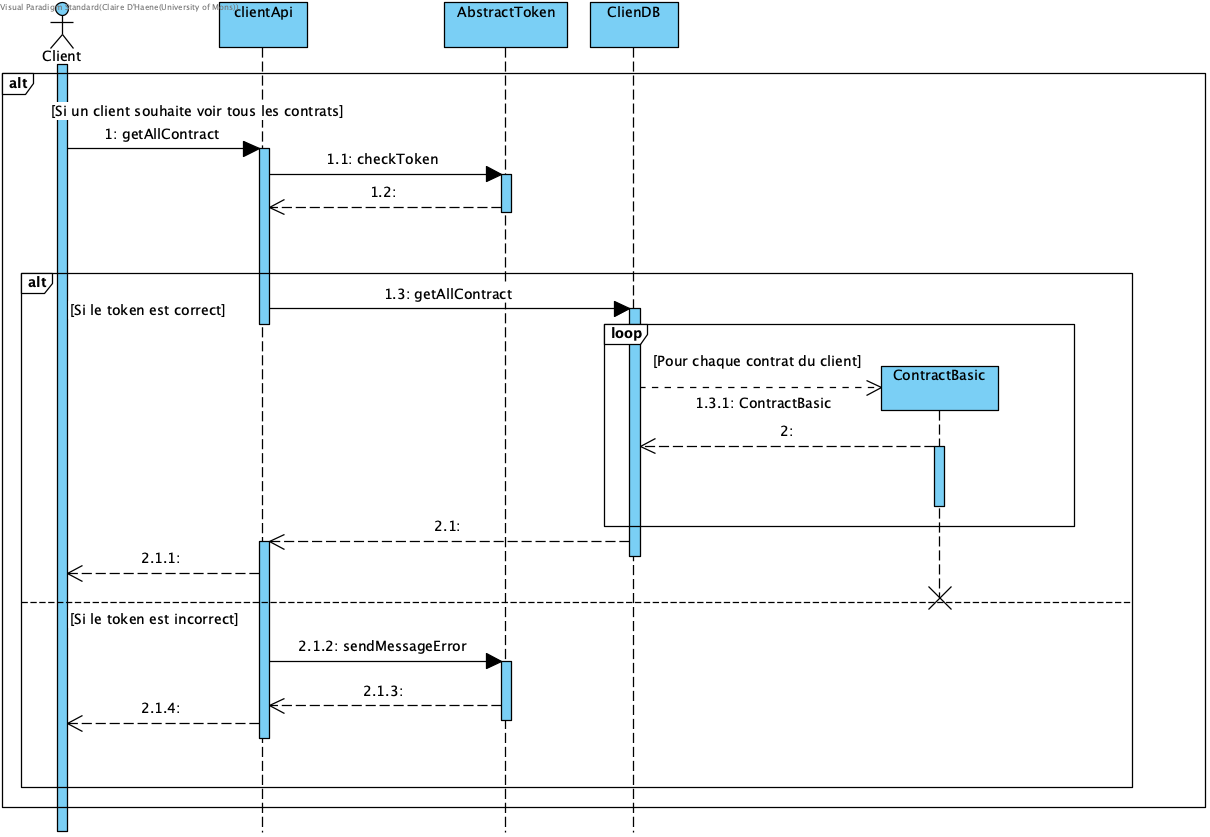
\includegraphics[width = 1\textwidth]{sequence/client/seqContrats.png}
\end{figure}

\newpage

\begin{flushleft}
Continuons avec l'Use Case \textbf{"Voir les fournisseurs et
contrats relatifs"}.
A cet effet, il y aura deux méthodes :
\end{flushleft}

\begin{enumerate}
\item getAllProposal si le client souhaite voir toutes les propositions.
\item getProposal si le client souhaite voir une proposition en particulier.
\end{enumerate}

\begin{flushleft}
Ces deux méthodes sont appelées une fois de clientApi et ensuite, une fois de ClientDB.
\end{flushleft}

\begin{flushleft}
Dans le cas de "getAllProposal", la valeur de retour est une ArrayList de "proposalBasic" donc nous utiliserons une boucle et dans le cas de "getProposal", nous devons simplement retourner une instance de "proposalFull".
\end{flushleft}

\begin{flushleft}
Concernant le Use Case \textbf{"Ajouter des contrats"}, nous appelons la méthode "clientProposeContract" de clientApi et ensuite, la méthode du même nom de ClientDB.
\end{flushleft}

\begin{flushleft}
Etant donné que cette dernière ne doit rien retourner, il n'y aura pas de valeur de retour.
\end{flushleft}

\newpage
\begin{figure}[h]
\centering
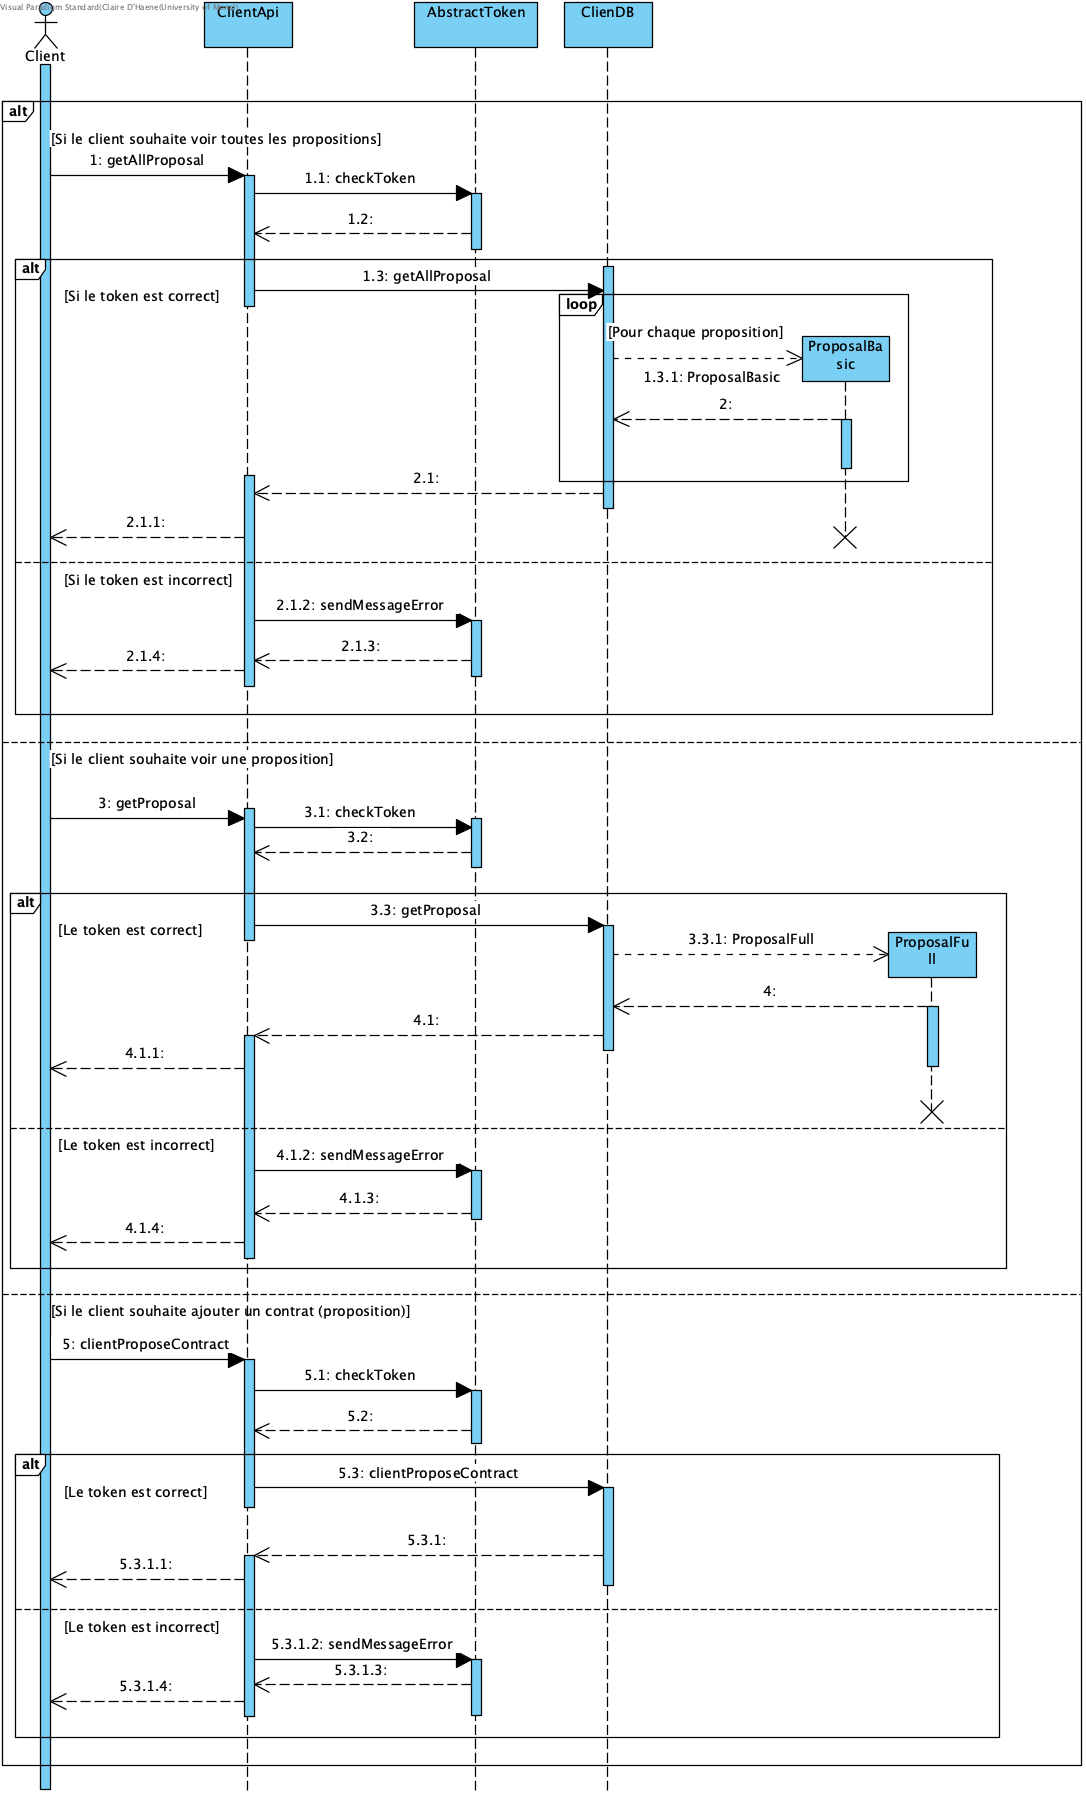
\includegraphics[width = 0.7\textwidth]{sequence/client/seqFCRe.png}
\end{figure}

\newpage
\begin{flushleft}
L'Use case \textbf{"Voir les portefeuilles"} fonctionne de la même manière qu'expliqué précédemment pour "Voir les fournisseurs et contrats relatifs".
En effet, il y aura deux méthodes : 
\end{flushleft}
\begin{enumerate}
\item getAllWallet si le client souhaite voir tous les portefeuilles. On doit donc retourner une ArrayList de "walletBasic".
\item getWallet si le client souhaite voir un portefeuille. On doit donc retourner une instance de "walletFull".
\end{enumerate}

\begin{flushleft}
Passons maintenant aux Use Cases \textbf{"Créer un portefeuille"} et \textbf{"Fermer un portefeuille"}.
\end{flushleft}

\begin{flushleft}
Pour \textbf{créer un portefeuille}, nous appelons donc la méthode "createWallet" de clientApi et ensuite, la méthode du même nom de ClientDB.
\end{flushleft}

\begin{flushleft}
Nous créons une instance de "walletBasic", que nous devons enregistrer dans "ClientDB" avant de clôturer l'exécution de la méthode car il s'agit d'un nouveau portefeuille à stocker.
\end{flushleft}

\begin{flushleft}
Pour \textbf{supprimer un portefeuille}, nous appelons la méthode "deleteWallet" de clientApi.
\end{flushleft}
\begin{flushleft}
Cependant, avant d'appeler la méthode du même nom de ClientDB, nous devons vérifier que le portefeuille est vide.
\end{flushleft}
\begin{flushleft}
Si c'est le cas le portefeuille sera bien supprimé, sinon, on renverra une erreur.
\end{flushleft}

\newpage
\begin{figure}[h]
\centering
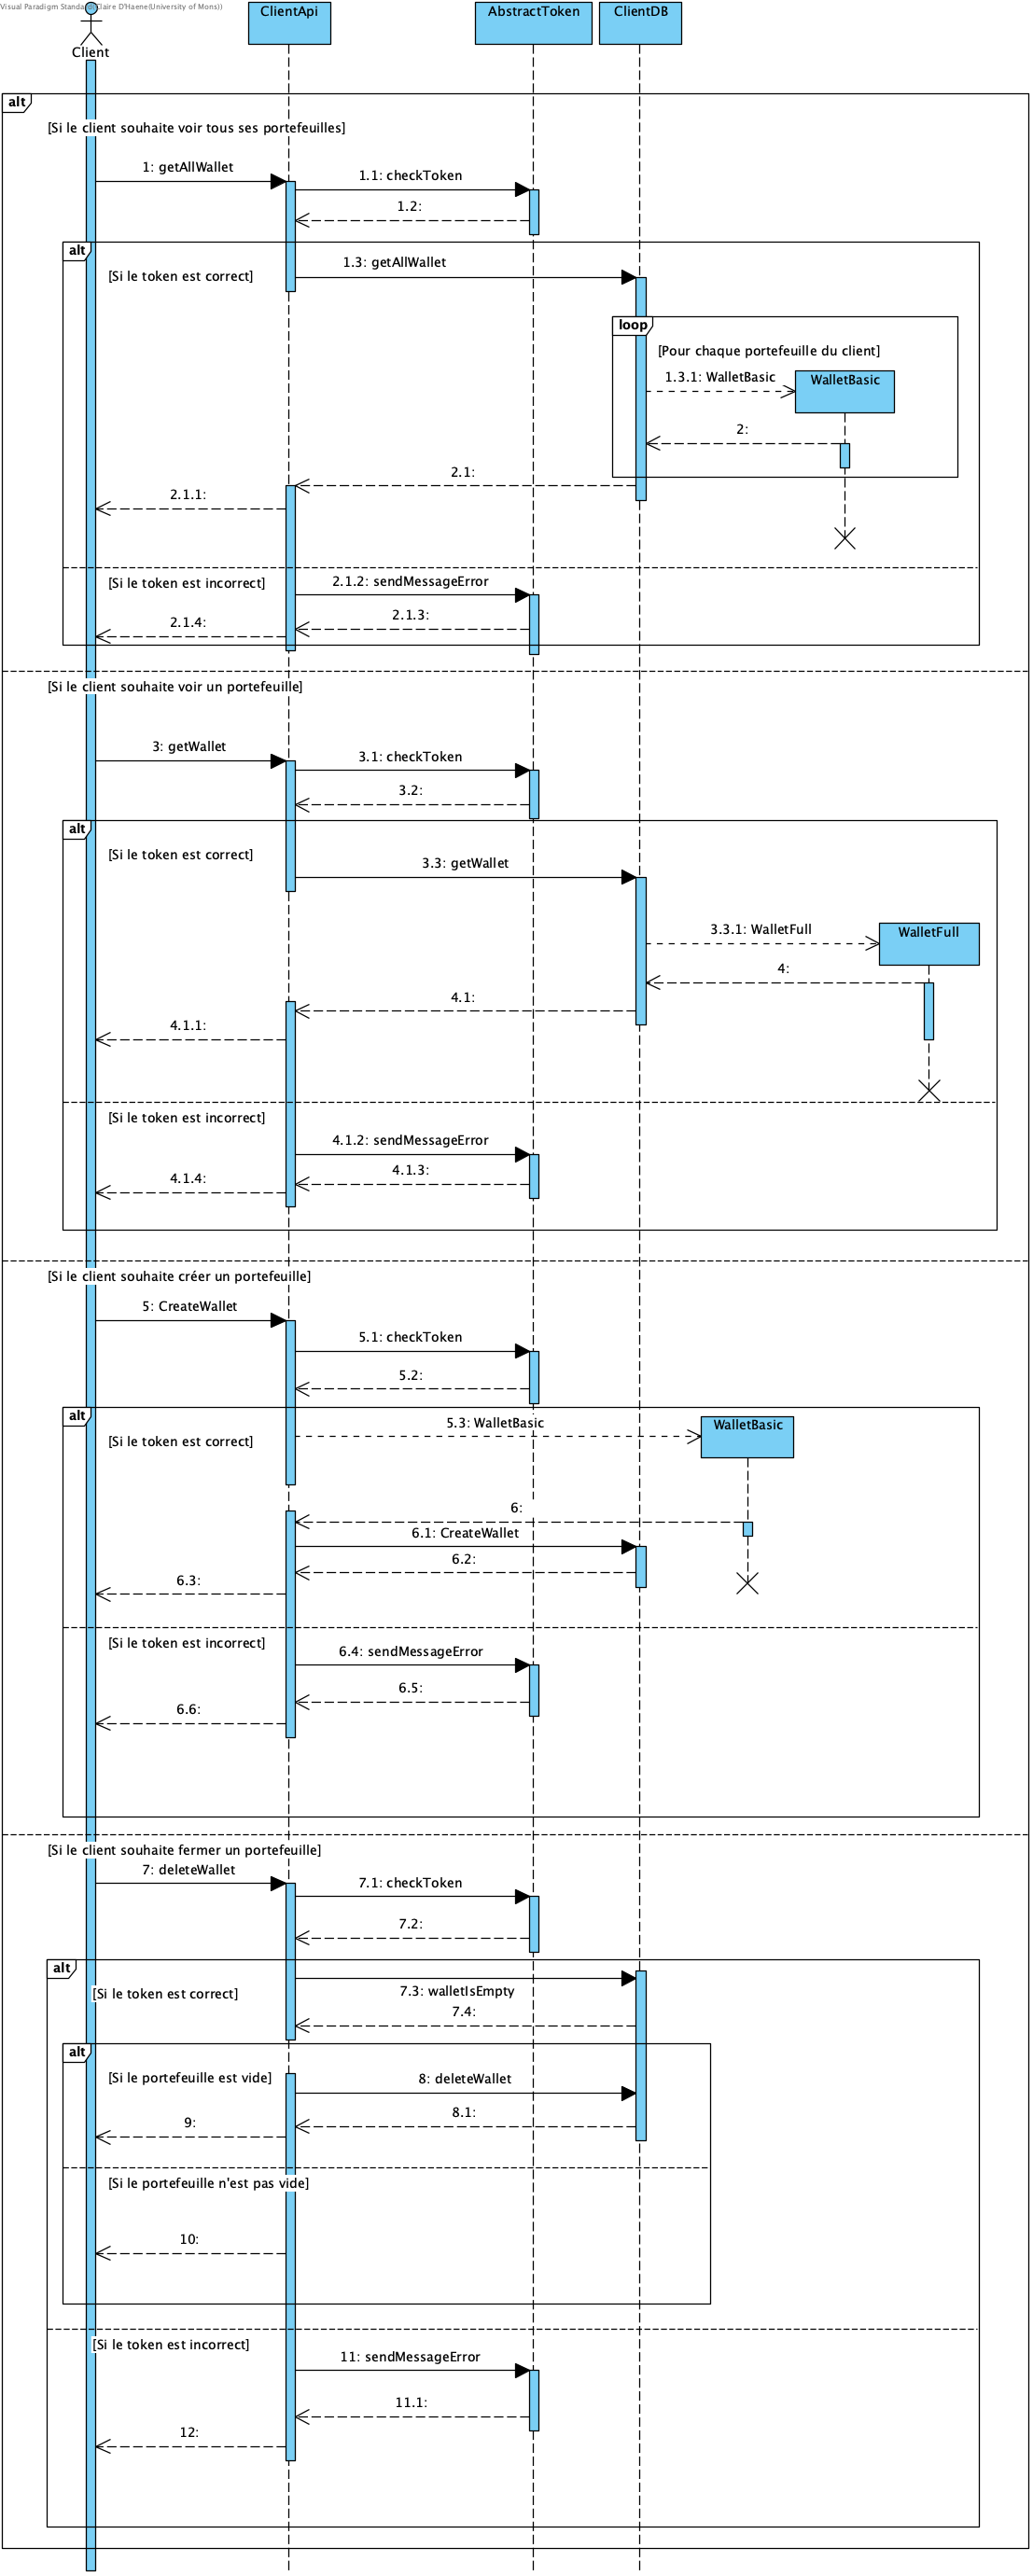
\includegraphics[width = 0.49\textwidth]{sequence/client/seqPortefeuilles.png}
\end{figure}

\newpage
\subsection{Provider}